\documentclass[12pt]{article}
\usepackage{amssymb, amsmath, amsfonts, bm, graphicx, geometry}
\usepackage{tabularx, booktabs, float, enumitem, multicol, mathtools}
\usepackage{parskip} % Auto-manages paragraph spacing and removes indentations
\usepackage{siunitx}  % Eases typesetting of numbers and units

\geometry{margin=1in}

\begin{document}

% --- Header Block ---
\noindent
\textbf{MA-224} \hfill \textbf{Zeshui Song} \\
\textbf{HW 1 Part 2} \hfill \today
\vspace{2mm}
\hrule
\vspace{6mm}

% --- Body Content ---
\section*{Section 1.1}
\textbf{10)} The experiment will be run 20 times. For each of the 20 trials, the sample space is infinite since it could take an infinite number of tries to get the first head.
\[S = \{1,2,3,\dots\}\]
The p.m.f. is then given by:
\[f(1) = (1/2)^1,\quad f(2) = (1/2)^2,\quad f(3) = (1/2)^3, \quad \dots\]


\begin{center}
\renewcommand{\arraystretch}{1.4}
\begin{tabular}{lccccc}
\toprule
$x$ & $1$ & $2$ & $3$ & $\dots$ & $x$ \\
\midrule
$f(x)$ & $0.5$ & $0.25$ & $0.125$ & $\dots$ & $(1/2)^{x}$ \\
\bottomrule
\end{tabular}
\end{center}
Through experimentation, the resulting relative frequency table is given below:
\begin{table}[htbp]
    \centering
    \begin{tabular}{lcccccccc}
        \toprule
        \# of flips & 1   & 2    & 3   & 4 & 5    & 6    & 7 & 8    \\
        \midrule
        Freq.        & 10  & 5    & 2   & 0 & 1    & 1    & 0 & 1    \\
        Rel. Freq.    & 0.5 & 0.25 & 0.1 & 0 & 0.05 & 0.05 & 0 & 0.05 \\
        \bottomrule
    \end{tabular}
    \label{tab:flip_frequencies}
\end{table}\\
The experimental frequency histogram $h(x)$ is plotted against the theoretical p.m.f. $f(x) = (1/2)^x$ below:
\begin{center}
    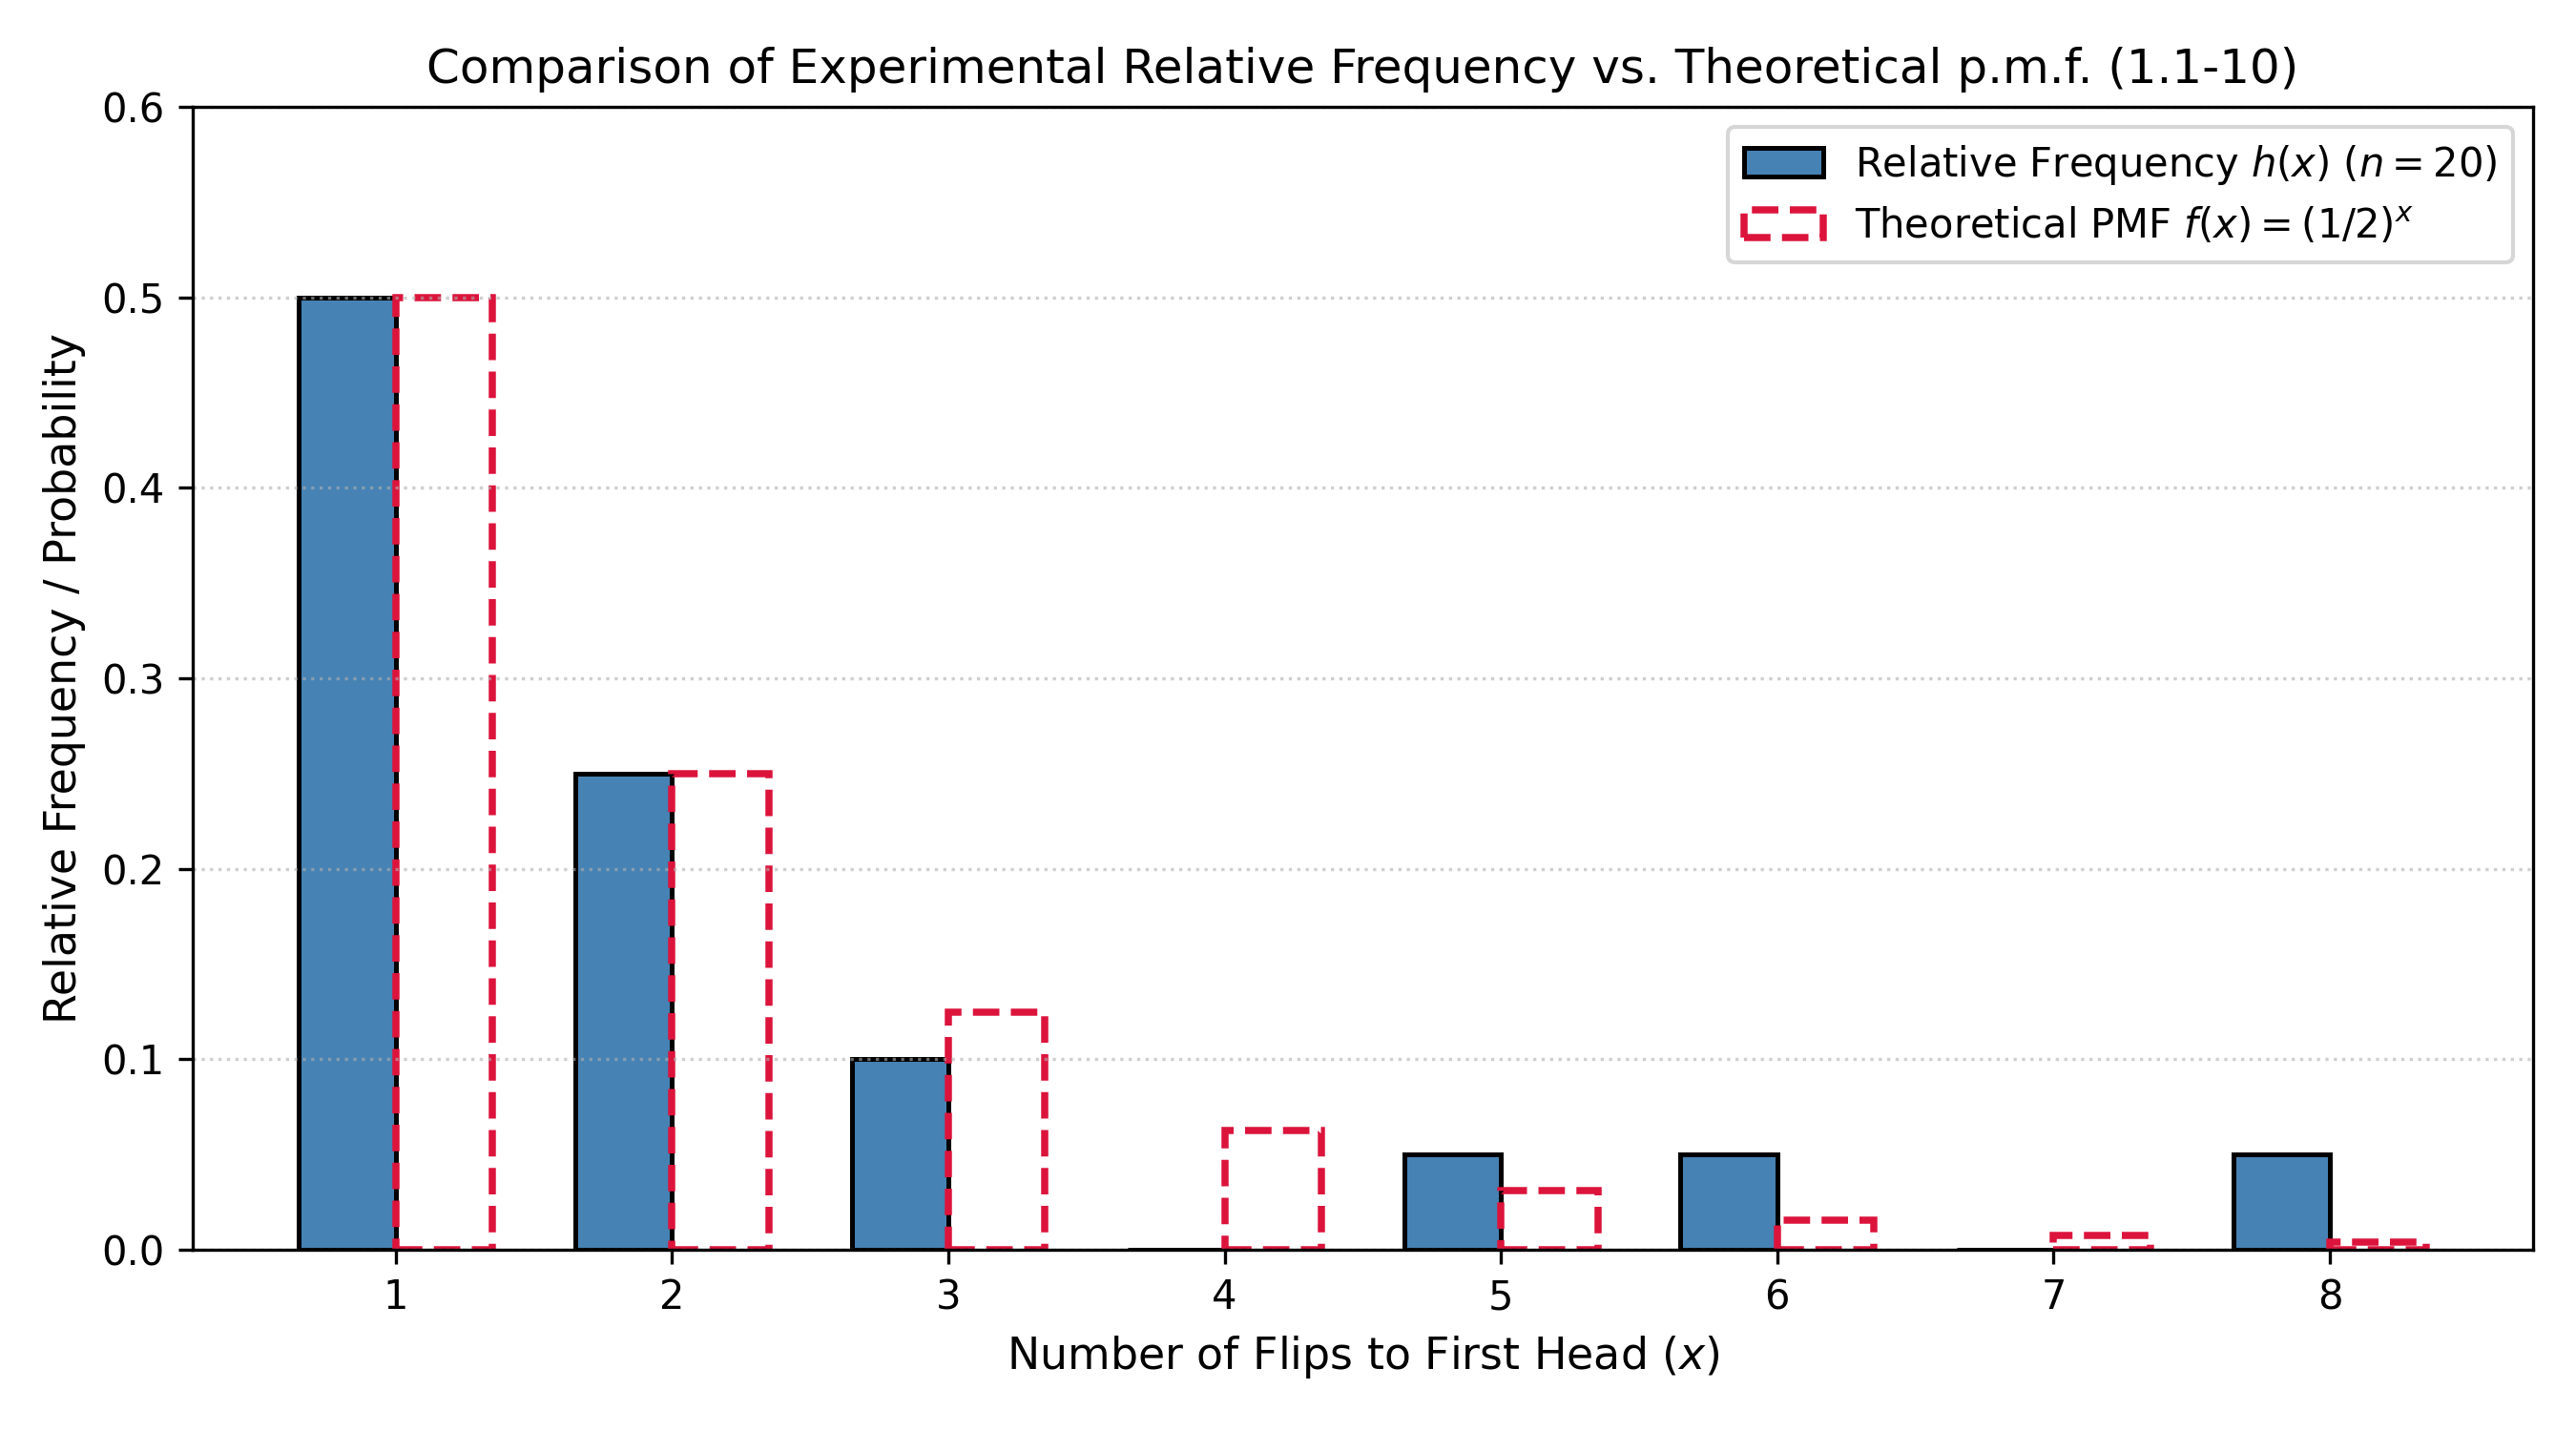
\includegraphics[width=0.8\textwidth]{histogram_pmf_comparison.png}
\end{center}
The experimental relative frequency $h(x)$ closely matches the theoretical p.m.f. $f(x) = (1/2)^x$ for low values of $x$ but starts to deviate for higher values of $x$ due to the limited number of trials.

\end{document}